% Vietnamese translation for OI Public Library
% Source-File: IOI中国国家候选队论文/2006/陈启峰/陈启峰.doc
\documentclass[11pt]{article}
\usepackage{oipl-vn}
\usepackage{tikz}
\usetikzlibrary{arrows.meta}

\newcommand{\Oh}{\mathcal{O}}

\title{Một căng một chùng, con đường giải bài}
\author{Chen Qifeng\\Trường Trung học Tưởng niệm Tôn Trung Sơn, Quảng Đông}
\date{2006}

\begin{document}
\maketitle

\origtitle{Applying constraining and relaxing methods in problem solving}
\sourcepath{IOI China candidate team papers / 2006 / Chen Qifeng.doc}

\renewcommand{\abstractname}{Tóm tắt}
\begin{abstract}
Bài viết trình bày cách dùng hai thao tác tư duy ``thêm ràng buộc'' và
``nới điều kiện'' trong thiết kế thuật toán. Phần đầu giải thích ý nghĩa của
hai phương pháp. Phần tiếp theo phân tích vì sao khi giải bài ta thường cần
thu hẹp hoặc mở rộng điều kiện. Ba ví dụ \textit{Kỵ sĩ}, \textit{Những loài
vật thân thiện} và \textit{Trạm cứu hỏa} lần lượt minh họa vai trò của thêm
ràng buộc, nới điều kiện, và phối hợp cả hai. Cuối cùng, tác giả tổng kết một
số kinh nghiệm để vận dụng linh hoạt hai phương pháp này.
\end{abstract}

\noindent\textbf{Từ khóa:} thêm ràng buộc; nới điều kiện; điều kiện quá rộng;
điều kiện quá phức tạp; điều kiện quá độc lập; điều kiện quá nghiêm ngặt.

\section{Định nghĩa}

\term{Phương pháp thêm ràng buộc} là chủ động thêm vào một số điều kiện hoặc
giới hạn, đồng thời chứng minh rằng dưới các điều kiện mới ấy vẫn tìm được
nghiệm cần thiết.

\term{Phương pháp nới điều kiện} là bỏ bớt hoặc làm yếu một số điều kiện, đồng
thời chứng minh rằng trong bài toán đã nới lỏng vẫn có thể tìm được nghiệm
tương ứng với yêu cầu ban đầu.

\section{Dẫn nhập}

Khi phân tích bài toán và thiết kế thuật toán, ta thường gặp hai kiểu bế tắc.
Một mặt, điều kiện có thể quá phức tạp hoặc quá nghiêm ngặt, khiến trạng thái
và quan hệ chuyển tiếp không thể viết ra. Mặt khác, điều kiện cũng có thể quá
rộng hoặc các đối tượng quá độc lập, khiến không biết nên bắt đầu từ đâu.

Lúc đó ta có thể thử hai thao tác trái chiều. Thêm ràng buộc giúp thu nhỏ phạm
vi nghiên cứu, làm lộ ra cấu trúc có thể khai thác. Nới điều kiện giúp bỏ một
lớp chi tiết đang cản trở, để trước hết nhìn thấy bài toán cốt lõi. Nếu dùng
khéo, hai thao tác này có thể đưa một bài toán tưởng như rối rắm về một mô
hình rõ ràng.

Các phần sau chọn ba bài toán tiêu biểu. Bài \textit{Kỵ sĩ} cho thấy cách thêm
ràng buộc để biến một không gian tìm kiếm vô hạn thành các phép tính số học.
Bài \textit{Những loài vật thân thiện} cho thấy cách nới một điều kiện thứ tự
quá khắt khe để thay cấu trúc dữ liệu phức tạp bằng quét tuyến tính. Bài
\textit{Trạm cứu hỏa} dùng cả hai: nới điều kiện để định nghĩa trạng thái quy
hoạch động, rồi thêm ràng buộc để có công thức chuyển tiếp.

\section{Ví dụ 1: Kỵ sĩ}

\subsection{Mô tả bài toán}

Một quân kỵ sĩ di chuyển trên bàn cờ vô hạn. Mỗi kiểu di chuyển được mô tả
bằng một cặp số nguyên \((a,b)\): từ \((x,y)\) có thể nhảy đến
\((x+a,y+b)\) hoặc \((x-a,y-b)\). Một kỵ sĩ có một danh sách hữu hạn các kiểu
nhảy. Đề bảo đảm tập các vị trí đến được không cùng nằm trên một đường thẳng.

Hai kỵ sĩ được gọi là tương đương nếu, bắt đầu từ \((0,0)\), tập tất cả các
vị trí mà chúng có thể đến được là như nhau. Có thể chứng minh rằng với mọi
kỵ sĩ đều tồn tại một kỵ sĩ tương đương chỉ có hai kiểu nhảy. Nhiệm vụ là tìm
hai cặp số nguyên như vậy.

\subsection{Mô hình và hướng tổng quát}

Xem mỗi kiểu nhảy là một vectơ nguyên \(v_i=(x_i,y_i)\). Tập các điểm đến được
là
\[
  \left\{\sum_{i=1}^{n} c_i v_i : c_i\in\mathbb{Z}\right\}.
\]
Ta cần tìm hai vectơ \(p,q\) sinh đúng cùng tập điểm.

Liệt kê hai vectơ cần tìm rồi kiểm tra bằng tìm kiếm theo bề rộng là không khả
thi, vì phạm vi tọa độ và bàn cờ đều vô hạn. Các hướng tham lam, quy hoạch
động hay đồ thị thông thường cũng không phù hợp. Bản chất của bài toán là biến
đổi tập sinh của một lưới nguyên, nên phải dùng lập luận số học.

Một ràng buộc quan trọng là: thay vì tìm trực tiếp hai vectơ từ \(n\) vectơ,
ta chỉ cần giải bài toán ``biến ba thành hai''. Nếu ba vectơ bất kỳ đều có thể
được thay bằng hai vectơ tương đương, thì với \(n>2\) vectơ ta lặp thao tác
này để giảm số vectơ đi một cho đến khi chỉ còn hai vectơ.

\subsection{Thêm ràng buộc cho bài toán con}

Ngay cả bài toán ``biến ba thành hai'' vẫn còn rộng. Ta tiếp tục thêm ràng
buộc cho một nhiệm vụ nhỏ hơn: với hai vectơ, hãy biến chúng thành hai vectơ
tương đương trong đó một vectơ là vectơ thẳng đứng.

Xét hai vectơ không cùng phương
\[
  p=(a,b),\qquad q=(c,d).
\]
Đặt
\[
  g=\gcd(a,c),\qquad \Delta=ad-bc.
\]
Nếu một vectơ đã thẳng đứng thì ta giữ dạng đó. Ngược lại, dùng Euclid mở
rộng tìm \(s,t\in\mathbb{Z}\) sao cho
\[
  sa+tc=g.
\]
Khi đó
\[
  r=sp+tq=(g,sb+td)
\]
là một vectơ trong lưới ban đầu có hoành độ \(g\). Các điểm của lưới trên cùng
một đường thẳng đứng xuất hiện theo chu kỳ
\[
  h=\frac{|\Delta|}{g}.
\]
Do đó cặp
\[
  r=(g,sb+td),\qquad z=(0,h)
\]
sinh đúng cùng lưới với \(p,q\).

Nguồn gốc dùng hình vẽ cho ví dụ \((2,3)\) và \((4,2)\). Sơ đồ dưới đây phục
dựng kết luận quan sát được:
\begin{enumerate}
  \item các điểm chỉ nằm trên những đường thẳng đứng có hoành độ là bội của
  \(g\);
  \item trên trục \(Oy\), các điểm xuất hiện cách nhau \(h\) đơn vị;
  \item các điểm trên các đường thẳng đứng khác thu được bằng cách tịnh tiến
  mẫu trên trục \(Oy\) bởi vectơ \(r\).
\end{enumerate}

\begin{figure}[ht]
\centering
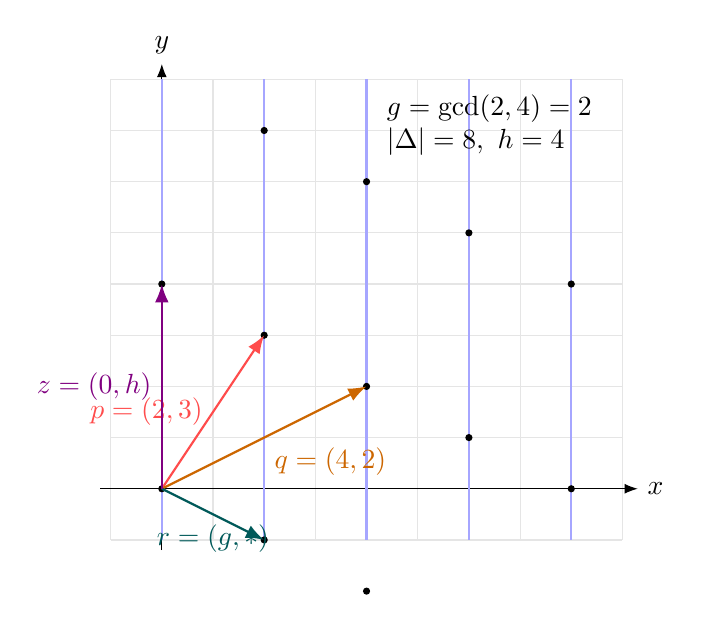
\begin{tikzpicture}[scale=0.65, >=Latex]
  \draw[step=1, gray!20] (-1,-1) grid (9,8);
  \draw[->] (-1.2,0) -- (9.3,0) node[right] {\(x\)};
  \draw[->] (0,-1.2) -- (0,8.3) node[above] {\(y\)};
  \foreach \x in {0,2,4,6,8} {
    \draw[blue!35, thick] (\x,-1) -- (\x,8);
  }
  \foreach \x/\y in {0/0,2/3,4/2,2/-1,0/4,2/7,4/6,6/5,8/4,4/-2,6/1,8/0} {
    \fill[black] (\x,\y) circle (2pt);
  }
  \draw[->, thick, red!70] (0,0) -- (2,3) node[midway, left] {\(p=(2,3)\)};
  \draw[->, thick, orange!80!black] (0,0) -- (4,2) node[midway, below right] {\(q=(4,2)\)};
  \draw[->, thick, teal!70!black] (0,0) -- (2,-1) node[midway, below] {\(r=(g,*)\)};
  \draw[->, thick, violet] (0,0) -- (0,4) node[midway, left] {\(z=(0,h)\)};
  \node[align=left] at (6.4,7.1)
    {\(g=\gcd(2,4)=2\)\\\(|\Delta|=8,\ h=4\)};
\end{tikzpicture}
\caption{Ví dụ lưới sinh bởi \((2,3)\) và \((4,2)\): các điểm nằm trên các đường \(x\) là bội của \(g\), còn chu kỳ theo phương dọc là \(h=|\Delta|/g\).}
\end{figure}

Chứng minh điểm mấu chốt cũng rất ngắn. Nếu một tổ hợp
\(\alpha p+\beta q\) có hoành độ \(0\), thì
\[
  \alpha a+\beta c=0.
\]
Vì \(g=\gcd(a,c)\), tồn tại \(m\in\mathbb{Z}\) sao cho
\[
  \alpha=m\frac{c}{g},\qquad \beta=-m\frac{a}{g}.
\]
Tung độ của tổ hợp đó là
\[
  \alpha b+\beta d
  =m\frac{cb-ad}{g},
\]
nên đúng là bội của \(h\). Chiều ngược lại cũng thu được từ tổ hợp nguyên
tương ứng. Vì vậy vectơ thẳng đứng \(z=(0,h)\) mô tả chính xác chu kỳ theo
phương dọc.

\subsection{Quay lại bài toán ban đầu}

Với ba vectơ \(v_1,v_2,v_3\), ta làm lần lượt:
\begin{enumerate}
  \item biến \(v_1,v_2\) thành một cặp tương đương gồm một vectơ thẳng đứng và
  một vectơ còn lại;
  \item ghép vectơ thẳng đứng vừa có với \(v_3\), rồi tiếp tục chuẩn hóa thành
  một cặp tương đương;
  \item trong ba vectơ trung gian còn lại, nếu một vectơ sinh được từ hai vectơ
  kia thì bỏ nó; nếu không, dùng lại phép chuẩn hóa để thu được hai vectơ sinh
  tương đương.
\end{enumerate}

Lặp quy trình ``ba thành hai'' trên danh sách ban đầu. Mỗi lần chỉ cần tính
\(\gcd\) và Euclid mở rộng, nên tổng thời gian là \(\Oh(n\log M)\), với \(M\)
là độ lớn tọa độ đang xét; bộ nhớ phụ là \(\Oh(1)\).

Điểm đáng chú ý không phải là công thức riêng lẻ, mà là chuỗi ràng buộc hợp
lý. Ta ràng buộc thuật toán phải giảm ba vectơ thành hai; ràng buộc phép biến
đổi hai vectơ phải tạo một vectơ thẳng đứng; rồi trong chứng minh tiếp tục cố
định hoành độ hoặc xét riêng trục \(Oy\). Chính các ràng buộc ấy làm bài toán
từ mơ hồ trở nên tính được.

\section{Ví dụ 2: Những loài vật thân thiện}

\subsection{Mô tả bài toán}

Trên hành tinh \(W\), mỗi loài sinh vật có \(k\) thuộc tính định lượng. Với
\(k-1\) thuộc tính đầu, hai loài càng khác nhau thì càng thân thiện; riêng
thuộc tính thứ \(k\), hai loài càng giống nhau thì càng thân thiện. Nếu
\(A_{a,i}\) là thuộc tính thứ \(i\) của loài \(a\), mức thân thiện được đo bởi
\[
  \operatorname{Friendliness}(a,b)=
  \sum_{i=1}^{k-1} C_i\lvert A_{a,i}-A_{b,i}\rvert
  - C_k\lvert A_{a,k}-A_{b,k}\rvert,
\]
trong đó các \(C_i\) không âm. Cần tìm cặp loài có mức thân thiện lớn nhất.

\subsection{Mâu thuẫn của cách tối ưu trực tiếp}

Liệt kê mọi cặp loài tốn \(\Oh(n^2k)\), không đủ nhanh. Vì \(k\le 5\), ta thử
bỏ trị tuyệt đối bằng cách liệt kê mẫu dấu. Với mỗi mẫu dấu \(BN\), đặt
\[
  F(a,BN)=\sum_{i=1}^{k}\operatorname{SIGN}(BN,i)C_iA_{a,i},
\]
trong đó \(\operatorname{SIGN}(BN,i)\in\{-1,1\}\). Giá trị cần xét có dạng
\[
  F(b,BN)-F(a,BN).
\]
Nhưng mẫu dấu chỉ hợp lệ nếu nó phù hợp với quan hệ lớn nhỏ của từng thuộc
tính:
\[
  \operatorname{SIGN}(BN,i)(A_{b,i}-A_{a,i})\ge 0
  \quad (1\le i\le k).
\]

Nếu giữ đủ điều kiện này, với mỗi loài \(a\) và mỗi mẫu dấu ta phải tìm một
loài \(b\) nằm trong một miền trực giao \(k\) chiều và có \(F(b,BN)\) lớn
nhất. Có thể dùng các cây đoạn nhiều tầng, nhưng thời gian, bộ nhớ và độ phức
tạp cài đặt đều nặng. Mâu thuẫn cốt lõi là điều kiện thứ tự trên mọi thuộc
tính quá khắt khe.

\subsection{Nới điều kiện}

Quan sát thuộc tính thứ \(k\) là thuộc tính duy nhất bị trừ trong hàm mục tiêu.
Vì vậy ta nới điều kiện: chỉ giữ đúng thứ tự ở thuộc tính thứ \(k\),
\[
  \operatorname{SIGN}(BN,k)(A_{b,k}-A_{a,k})\ge 0,
\]
còn các thuộc tính \(1,\ldots,k-1\) để việc liệt kê mẫu dấu tự chọn phương án
tốt nhất.

Cách nới này không làm thay đổi đáp án. Thật vậy, với mọi \(A,B\in\mathbb{R}\),
\[
  |A-B|\ge A-B,\qquad |A-B|\ge B-A.
\]
Do đó nếu đã cố định đúng chiều của thuộc tính thứ \(k\), thì với mỗi cặp
\((a,b)\), việc lấy cực đại trên mọi dấu của các thuộc tính còn lại sẽ phục
hồi đúng tổng các trị tuyệt đối có dấu cộng. Nói cách khác, mọi bộ thỏa điều
kiện nới lỏng đều có một mẫu dấu hợp lệ hoàn toàn cho giá trị không nhỏ hơn.
Vì tập hợp hợp lệ ban đầu lại là con của tập hợp nới lỏng, hai cực đại bằng
nhau.

\subsection{Thuật toán sau khi nới điều kiện}

Sắp xếp các loài theo thuộc tính \(A_{\cdot,k}\) tăng dần. Khi quét theo thứ
tự này, điều kiện ở thuộc tính thứ \(k\) được bảo đảm bằng vị trí trong thứ tự
sắp xếp. Với mỗi mẫu dấu cần xét, duy trì giá trị tốt nhất của \(F(b,BN)\) đã
gặp; dùng hiệu \(F(b,BN)-F(a,BN)\) để cập nhật đáp án, rồi đưa loài hiện tại
vào cấu trúc tốt nhất.

Tính các giá trị \(F\) cho mọi mẫu dấu tốn \(\Oh(n2^k)\), sắp xếp tốn
\(\Oh(n\log n)\). Độ phức tạp tổng là
\[
  \Oh(n\log n+n2^k),
\]
với bộ nhớ \(\Oh(n2^k)\), hoặc \(\Oh(2^k)\) nếu tính theo dòng khi quét.

Từ ví dụ này có thể rút ra một khuôn mẫu cho bài toán cực đại hoặc cực tiểu:
trước hết mô hình hóa, tìm thuật toán trực tiếp, thử tối ưu bằng cấu trúc dữ
liệu, rồi phân tích điều kiện nào đang làm cấu trúc trở nên nặng nề. Nếu điều
kiện đó có thể được thay bằng điều kiện yếu hơn mà không đổi giá trị tối ưu,
ta thường thu được lời giải đơn giản hơn nhiều.

\section{Ví dụ 3: Trạm cứu hỏa}

\subsection{Mô tả bài toán}

Quốc gia \(Z\) có \(n\) thành phố, giữa hai thành phố bất kỳ có đúng một đường
đi, nên mạng đường là một cây có trọng số. Xây trạm cứu hỏa tại thành phố
\(k\) tốn chi phí \(W_k\). Nếu thành phố \(u\) không có trạm, khoảng cách từ
\(u\) đến trạm gần nhất không được vượt quá \(D_u\). Trong phạm vi cho phép,
mỗi thành phố phải chọn trạm gần nhất làm trạm phụ trách. Cần cực tiểu hóa
tổng chi phí xây trạm.

Gọi \(\operatorname{dist}(u,v)\) là khoảng cách trên cây. Bài toán là chọn các
biến nhị phân \(x_v\) sao cho với mọi \(u\) tồn tại \(v\) thỏa
\[
  x_v=1,\qquad \operatorname{dist}(u,v)\le D_u,
\]
và \(\sum_v W_vx_v\) nhỏ nhất, đồng thời việc phụ trách phải tuân theo điều
kiện ``gần nhất''.

\subsection{Nới điều kiện để định nghĩa trạng thái}

Vì đồ thị là cây và mục tiêu là cực tiểu hóa, hướng tự nhiên là quy hoạch động
trên cây. Nhưng nếu trạng thái chỉ ghi chi phí nhỏ nhất trong cây con thì
không biết trạm nào phụ trách gốc cây con. Nếu thêm tham số là khoảng cách đến
trạm gần nhất, hoặc số hiệu trạm gần nhất trong hay ngoài cây con, chuyển tiếp
vẫn khó viết vì khái niệm ``gần nhất'' phải nhất quán khi ghép các cây con.

Rào cản chính là điều kiện quá nghiêm ngặt: thành phố phải chọn trạm gần nhất.
Thực ra để kiểm tra tính hợp lệ, ta chỉ cần biết trong bán kính \(D_u\) có ít
nhất một trạm. Vì vậy nới điều kiện thành: mỗi thành phố có thể chọn bất kỳ
trạm nào trong khoảng cách không quá \(D_u\) làm trạm phụ trách.

Giá trị tối ưu không đổi. Với một tập trạm đã xây hợp lệ theo điều kiện nới
lỏng, nếu một thành phố đang chọn một trạm không gần nhất, ta đổi nó sang trạm
gần nhất. Khoảng cách không tăng và chi phí xây trạm không đổi. Do đó luôn có
một phương án tối ưu của bài toán nới lỏng thỏa điều kiện ban đầu.

Gốc cây tại một đỉnh tùy ý. Ký hiệu \(T_i\) là cây con gốc \(i\). Định nghĩa
\(F(i,j)\) là chi phí nhỏ nhất để:
\begin{itemize}
  \item xây một số trạm trong \(T_i\);
  \item bảo đảm tại \(j\) có trạm;
  \item mọi đỉnh trong \(T_i\) chọn một trạm nằm trong \(T_i\) hoặc trạm tại
  \(j\), và khoảng cách không vượt quá giới hạn của nó;
  \item riêng đỉnh \(i\) chọn trạm tại \(j\);
  \item nếu \(j\notin T_i\), chi phí xây trạm tại \(j\) không tính vào
  \(F(i,j)\).
\end{itemize}
Nhờ nới điều kiện, định nghĩa này không cần nhắc đến trạm gần nhất.

\subsection{Thêm ràng buộc để có chuyển tiếp}

Sau khi nới điều kiện, mỗi đỉnh được chọn trạm phụ trách khá tự do. Sự tự do
này lại làm chuyển tiếp thiếu cấu trúc. Ta thêm ràng buộc sau: nếu đỉnh \(u\)
chọn trạm tại \(v\), và đường đi từ \(u\) đến \(v\) là
\[
  u=p_0,p_1,\ldots,p_t=v,
\]
thì mọi đỉnh \(p_r\) trên đường đi cũng chọn trạm tại \(v\).

Cần chứng minh ràng buộc này không làm mất nghiệm tối ưu. Lấy một phương án
tối ưu bất kỳ. Thêm đỉnh ảo \(s\), nối \(s\) với mọi đỉnh có trạm bằng cạnh
trọng số \(0\), rồi chạy Dijkstra từ \(s\). Với mỗi đỉnh, chọn trạm phụ trách
theo tiền nhiệm trên cây đường đi ngắn nhất; các đỉnh có trạm chọn chính nó.
Khi đó mọi đỉnh trên đường về trạm đều chọn cùng trạm. Vì mỗi đỉnh được gán
đến một trạm gần nhất trong tập trạm đã xây, giới hạn \(D_u\) vẫn được thỏa,
và tập trạm xây không đổi. Vậy ràng buộc mới là hợp lệ.

\subsection{Chuyển tiếp quy hoạch động}

Đặt
\[
  G(i)=\min_j F(i,j),
\]
nghĩa là chi phí nhỏ nhất để giải hoàn toàn cây con \(T_i\) bằng các trạm nằm
trong cây con.

Nếu \(\operatorname{dist}(i,j)>D_i\), thì \(F(i,j)=+\infty\). Ngược lại có ba
trường hợp.

\paragraph{Trạm \(j\) nằm ngoài \(T_i\).}
Với mỗi con \(v\) của \(i\), cây con \(T_v\) hoặc tự giải bên trong với chi
phí \(G(v)\), hoặc để gốc \(v\) cũng chọn trạm ngoài \(j\) với chi phí
\(F(v,j)\). Vì vậy
\[
  F(i,j)=\sum_{v\in\operatorname{child}(i)}\min\{G(v),F(v,j)\}.
\]

\paragraph{\(j=i\).}
Ta trả thêm chi phí xây trạm tại \(i\):
\[
  F(i,i)=W_i+
  \sum_{v\in\operatorname{child}(i)}\min\{G(v),F(v,i)\}.
\]

\paragraph{\(j\in T_i\) và \(j\ne i\).}
Khi đó \(j\) nằm trong đúng một cây con \(T_c\) của một con \(c\) của \(i\).
Cây con ấy phải dùng \(F(c,j)\), còn các cây con khác chọn giữa tự giải và
chọn trạm \(j\):
\[
  F(i,j)=F(c,j)+
  \sum_{\substack{v\in\operatorname{child}(i)\\v\ne c}}
  \min\{G(v),F(v,j)\}.
\]

Sau khi tính \(F(i,j)\), lấy \(G(i)=\min_jF(i,j)\). Đáp án là \(G(r)\), với
\(r\) là gốc cây. Số trạng thái là \(\Oh(n^2)\); bản gốc nêu độ phức tạp theo
cách cài đặt và tiền xử lý khoảng cách tương ứng. Ý chính của lời giải nằm ở
việc nới điều kiện để trạng thái có nghĩa, rồi thêm ràng buộc đường đi để
chuyển tiếp không hậu nghiệm.

\section{Tổng kết}

Hai phương pháp ``thêm ràng buộc'' và ``nới điều kiện'' đều nhằm đơn giản hóa
bài toán, nhưng dùng trong hai tình huống khác nhau. Khi điều kiện quá rộng,
đối tượng quá độc lập, hoặc phạm vi tìm kiếm quá mơ hồ, ta thêm ràng buộc để
thu nhỏ không gian nghiên cứu. Khi điều kiện quá phức tạp hoặc quá nghiêm
ngặt, ta nới điều kiện để bỏ lớp chi tiết đang cản trở mô hình hóa.

Điều quan trọng là mọi thay đổi đều phải đi kèm chứng minh: thêm ràng buộc
không được làm mất toàn bộ nghiệm cần tìm, và nới điều kiện không được làm đổi
giá trị tối ưu hoặc làm mất khả năng quay lại bài toán gốc.

Một căng một chùng không chỉ là đạo lý trong văn võ, mà cũng là con đường giải
bài. Muốn dùng thành thạo, ngoài luyện tập còn cần giữ vài thói quen:
\begin{itemize}
  \item dám thử cách nhìn mới;
  \item dám đưa ra phỏng đoán rồi kiểm chứng;
  \item dám so sánh với bài toán hoặc thuật toán quen thuộc;
  \item dám mở rộng mô hình khi lời giải hiện tại còn quá hẹp.
\end{itemize}
Trong đó, tinh thần đổi mới đặc biệt quan trọng: chỉ khi liên tục thử nghiệm
và kiểm chứng, ta mới có thể tìm được cấu trúc ẩn sau bài toán.

\section*{Lời cảm ơn}

Tác giả chân thành cảm ơn thầy Xiang vì những hướng dẫn và góp ý; cảm ơn Guo
Huayang từ Trường Trung học Changjun vì đã giải đáp ví dụ thứ nhất; cảm ơn
Zhou Gelin, Guo Huayang và Yang Mu vì các ý kiến quý báu.

\end{document}
